RF, LUCCK, and SVM were trained on tensor-reduced ECG features, presented in Table \ref{fig:ecgonly}. We compare these models to those trained on tensor-reduced ECG features and arterial line features, presented in Table \ref{fig:sigonly}. These figures display the mean F1 Score and AUROC over 100 iterations, with error bars indicating one SD. The $x$-axis indicates the rank selected for CP-ALS, with the rightmost columns, separated with a dashed line, representing the case where no tensor decomposition was applied.

Figure \ref{fig:sigEHR} shows the results of models trained on both the tensor-reduced signal features and EHR data.

\begin{figure}[htb]
    \centering
    \begin{subfigure}[htb]{\textwidth}
        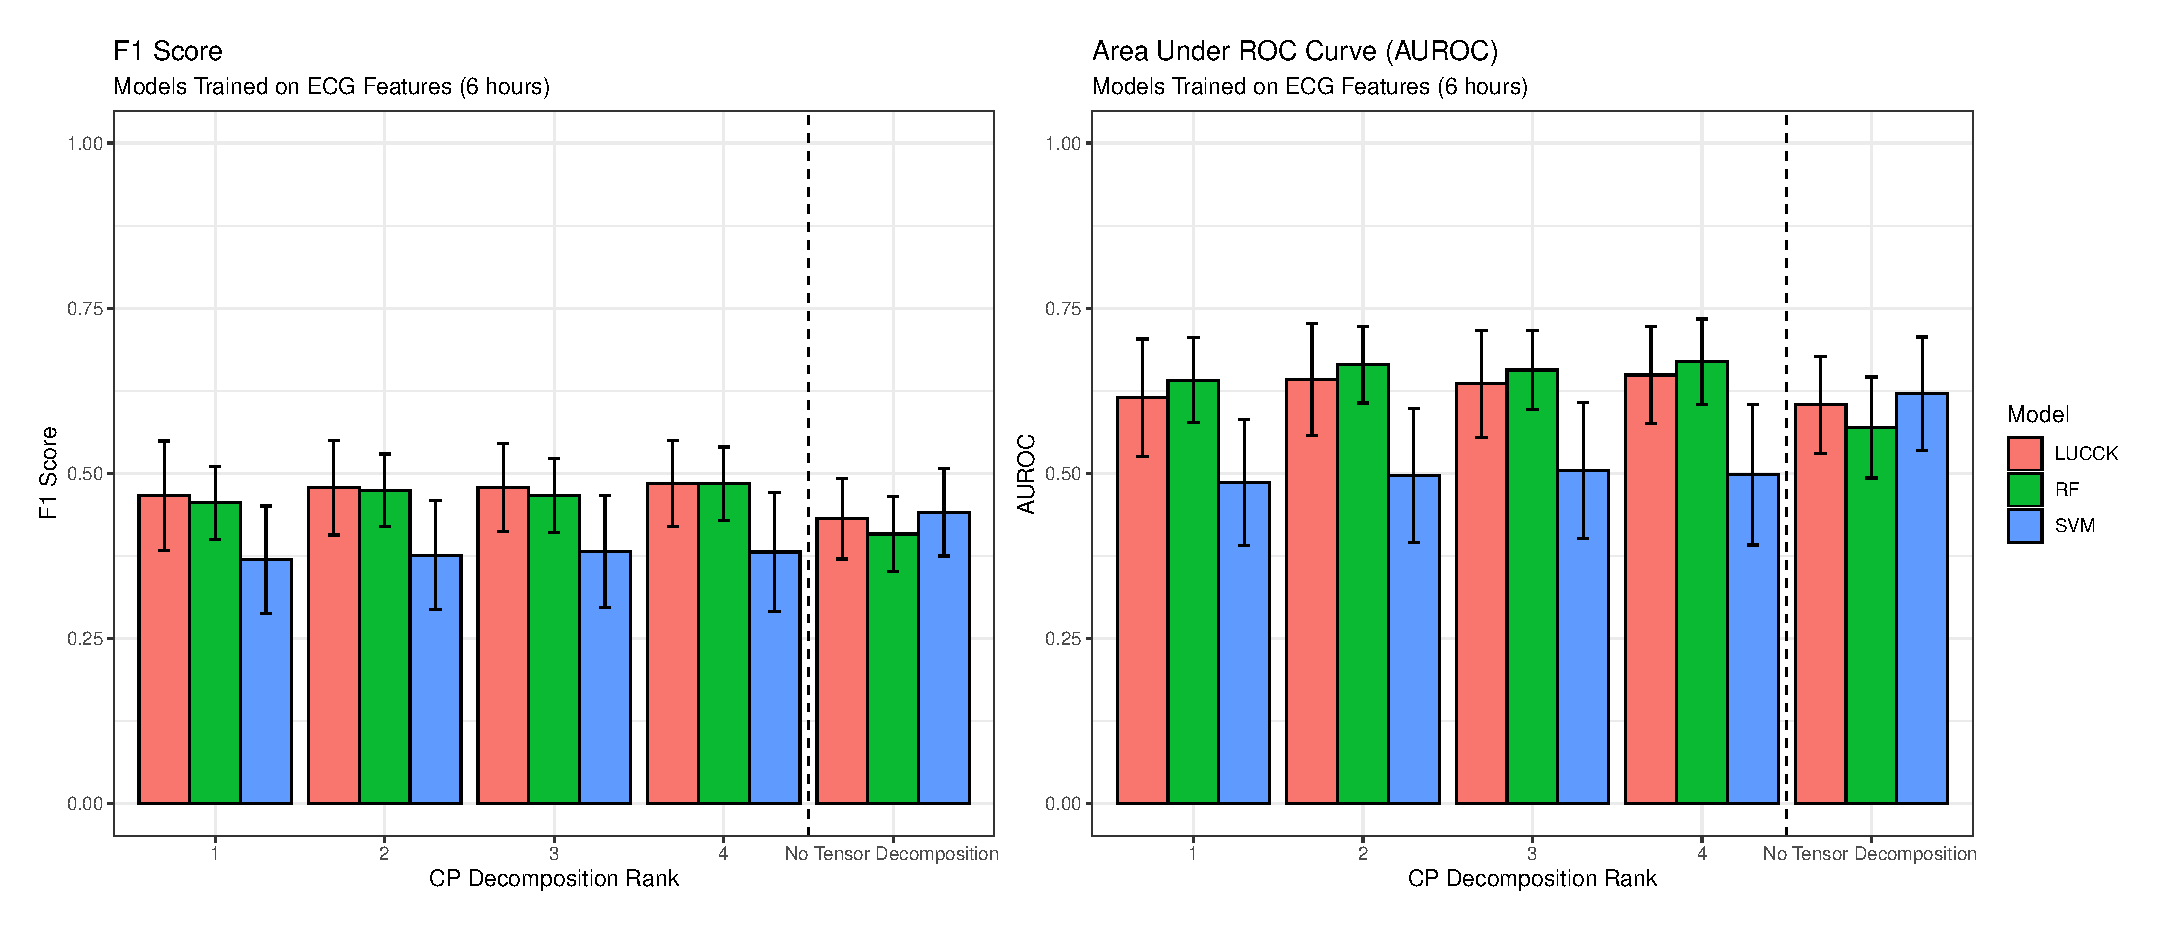
\includegraphics[width=\textwidth]{body/figures/ecg_6.eps}
        \caption{6-hour data}
    \end{subfigure}
    \hfill
    \begin{subfigure}[htb]{\textwidth}
        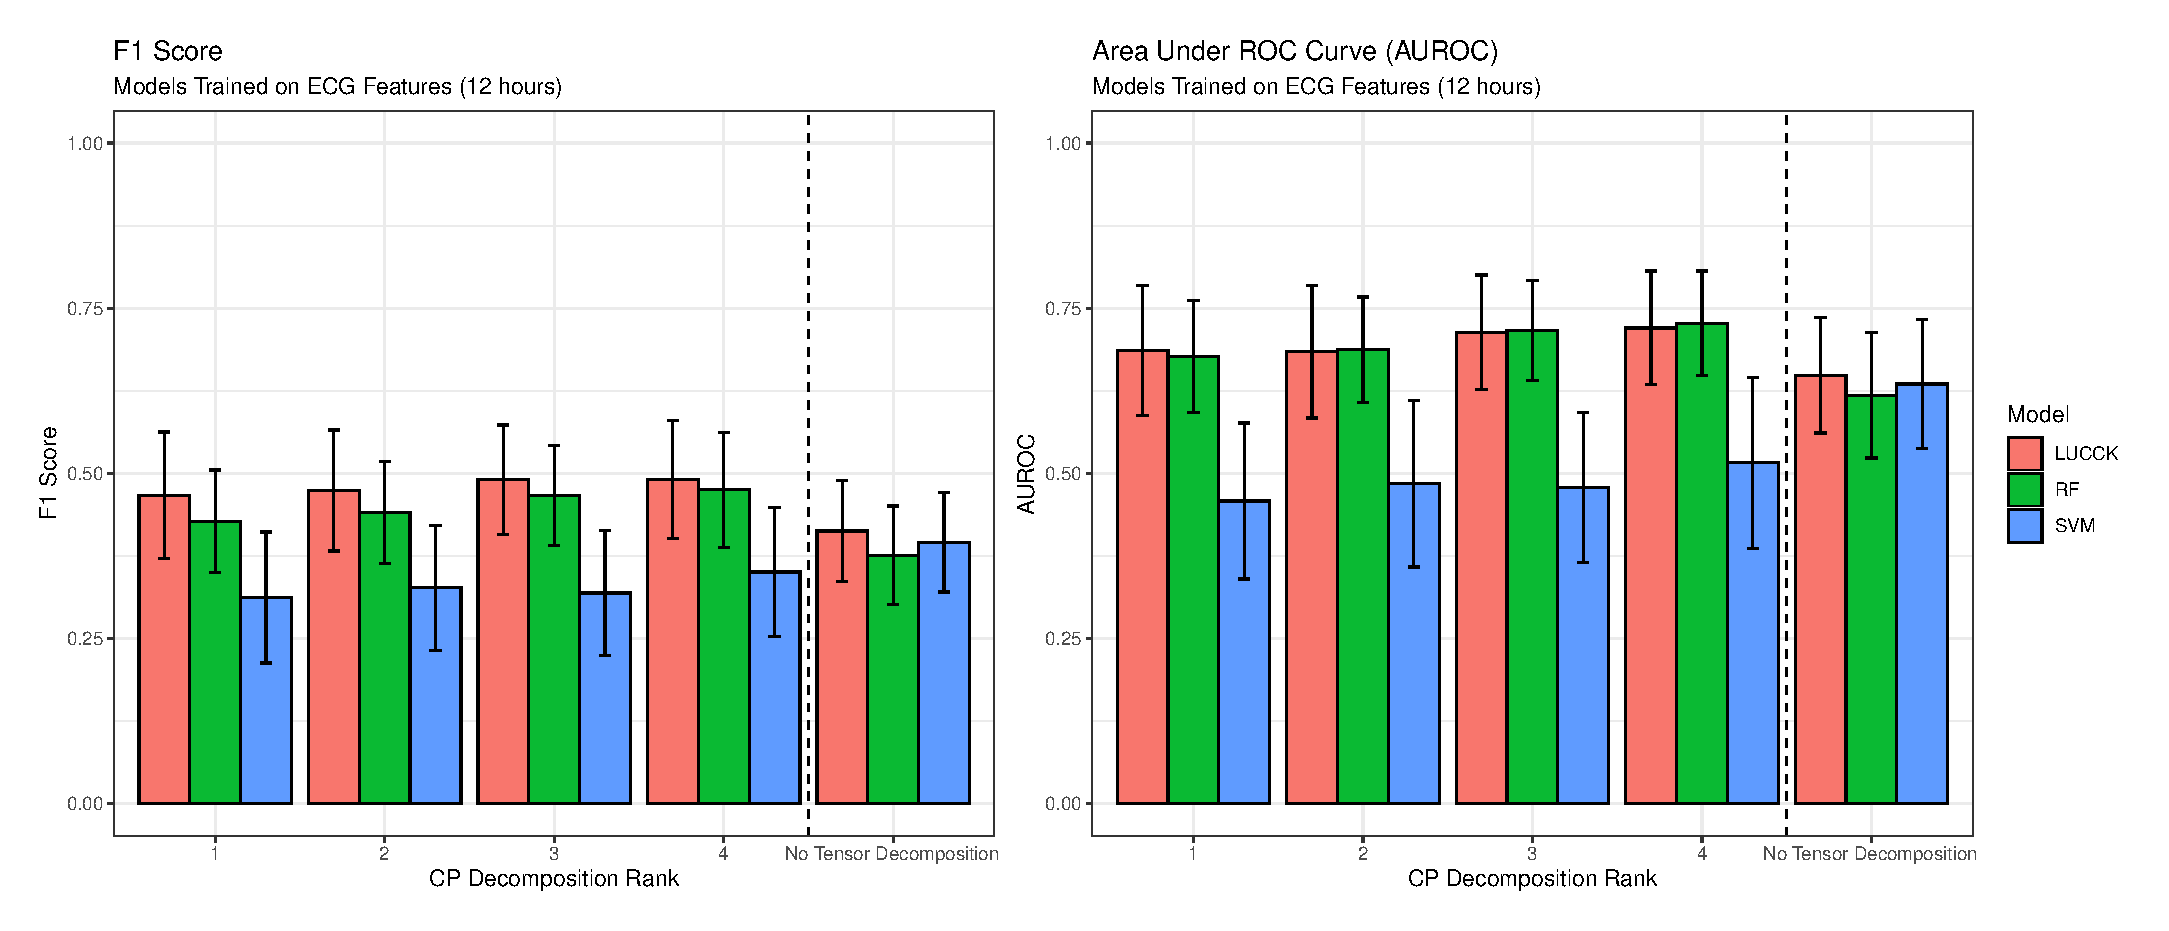
\includegraphics[width=\textwidth]{body/figures/ecg_12.eps}
        \caption{12-hour data}
    \end{subfigure}
    \caption{Models Trained with ECG}
    \label{fig:ecgonly}
\end{figure}  % ECG 

\begin{figure}[htb]
    \centering
    \begin{subfigure}[htb]{\textwidth}
        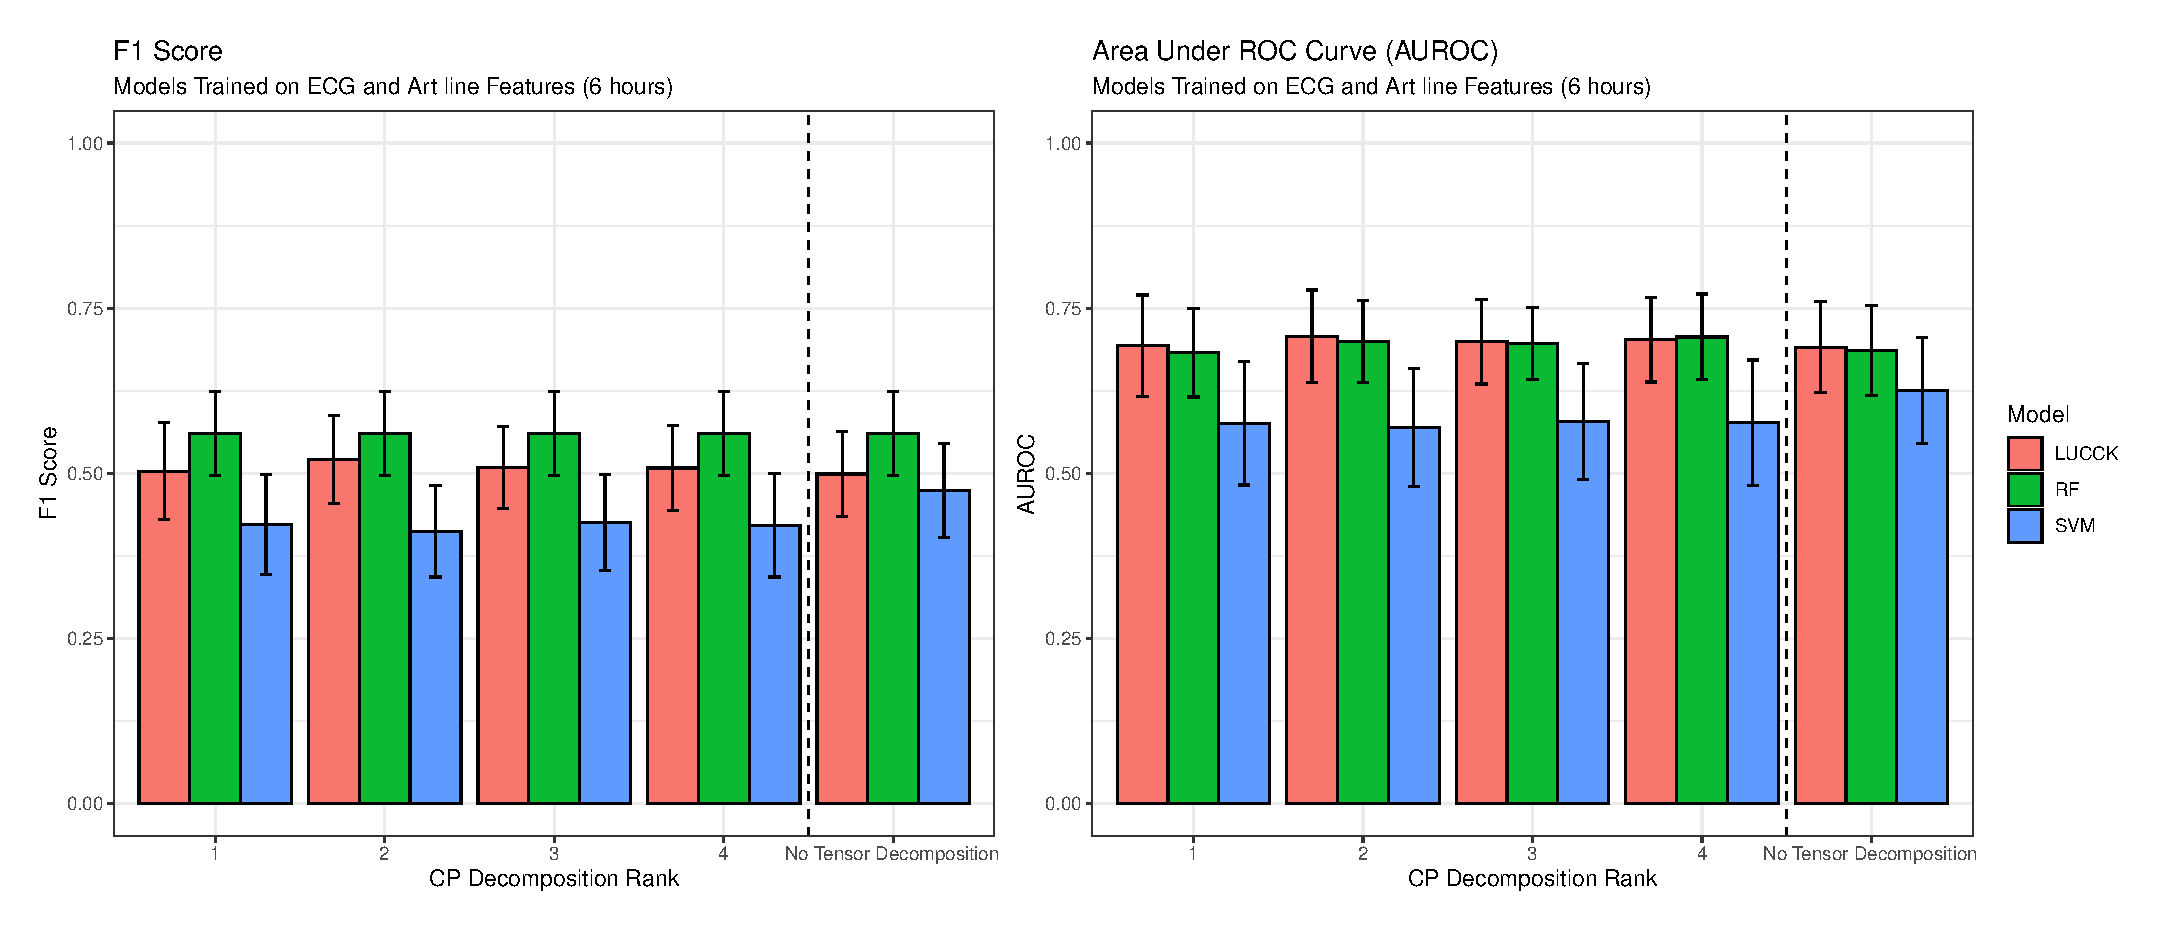
\includegraphics[width=\textwidth]{body/figures/both_6.eps}
        \caption{6-hour data}
    \end{subfigure}
    \hfill
    \begin{subfigure}[htb]{\textwidth}
        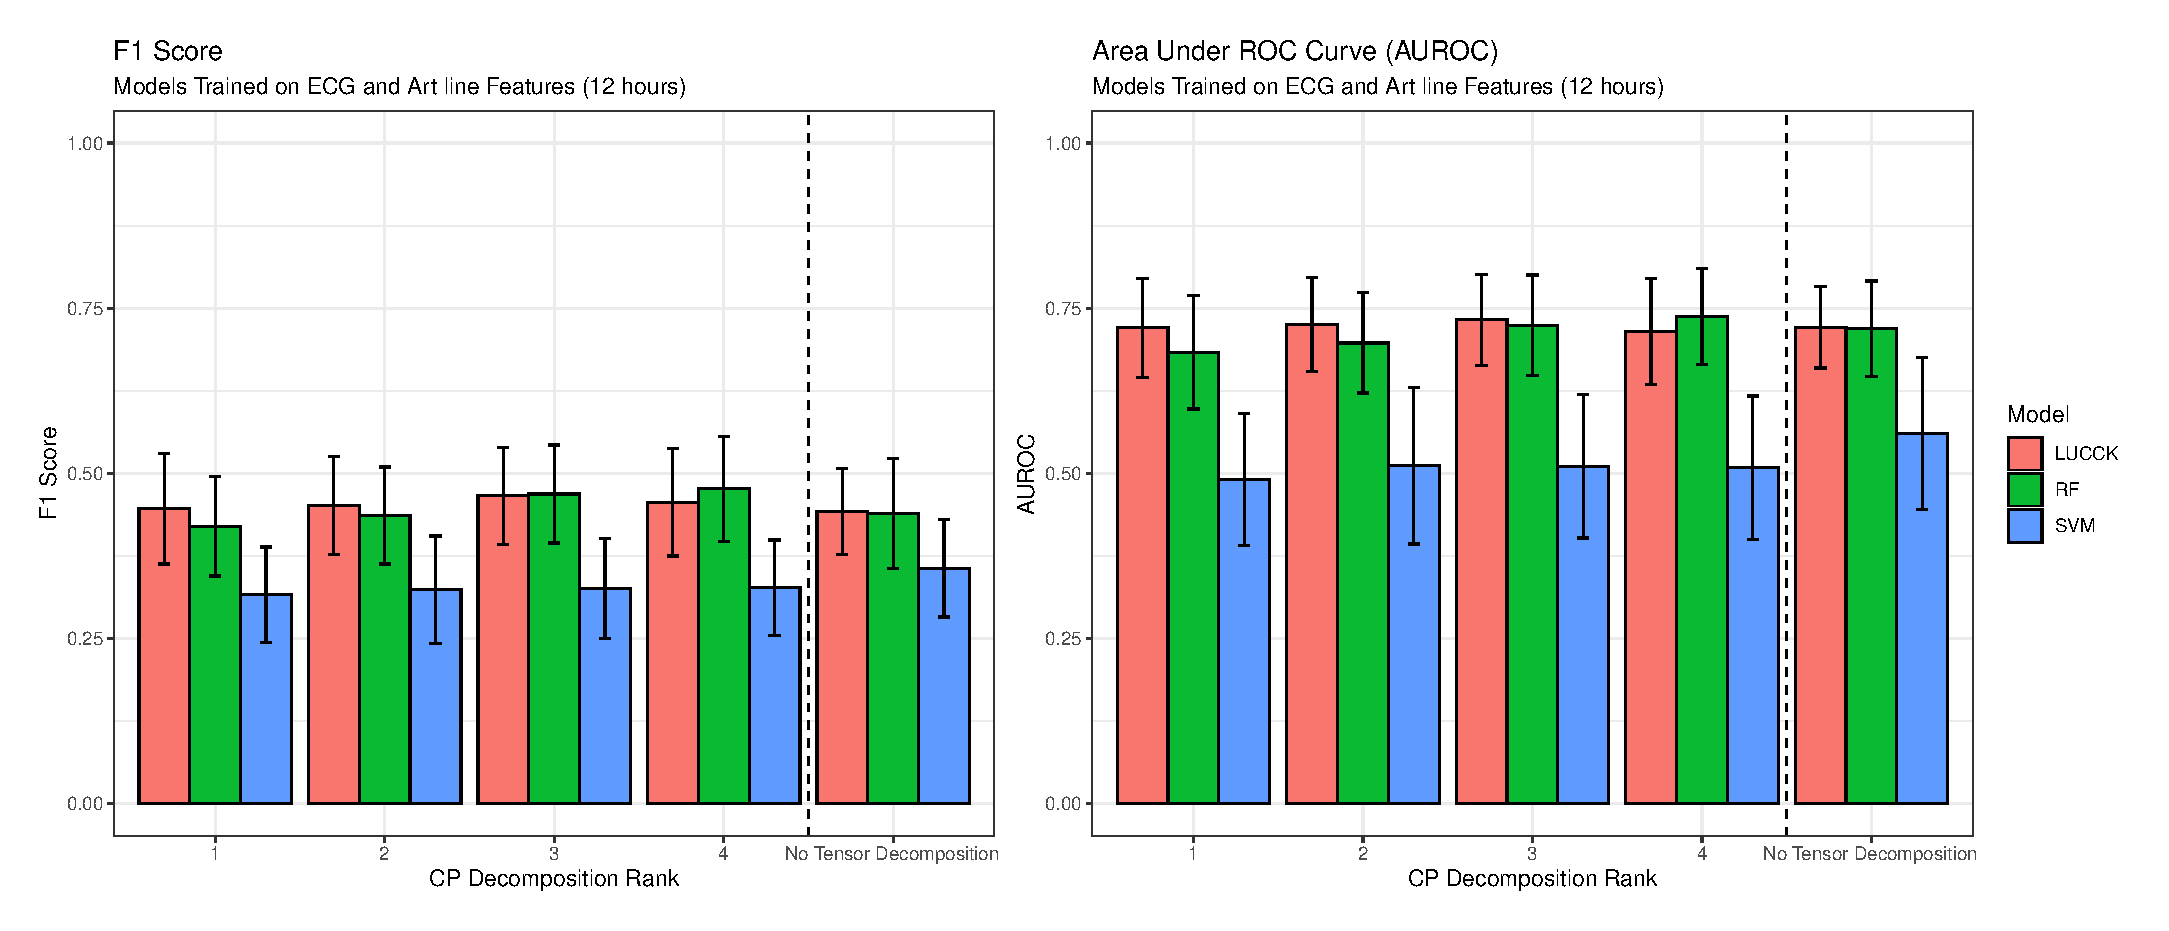
\includegraphics[width=\textwidth]{body/figures/both_12.eps}
        \caption{12-hour data}
    \end{subfigure}
    \caption{Models Trained with Arterial Line and ECG}
    \label{fig:sigonly}
\end{figure}  % ART + ECG 

\begin{figure}[htb]
    \centering
    \begin{subfigure}[htb]{\textwidth}
        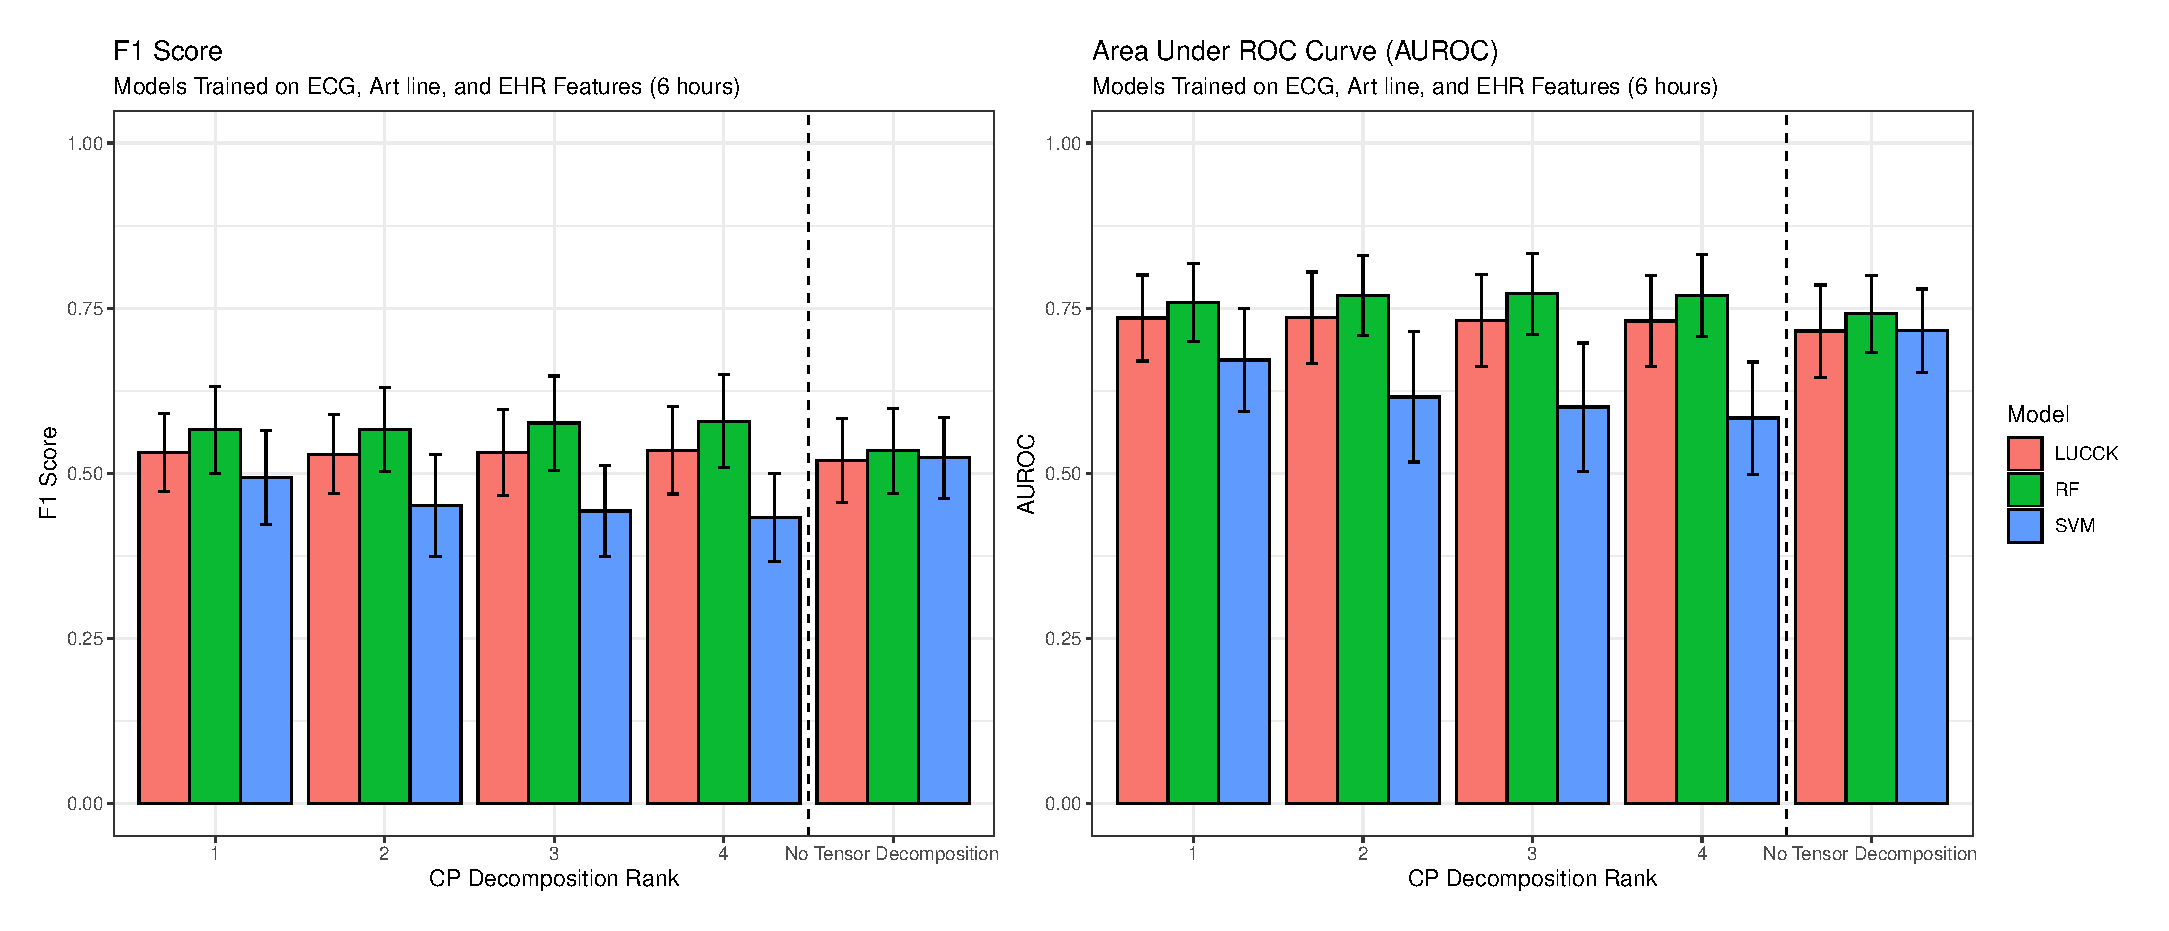
\includegraphics[width=\textwidth]{body/figures/all_6.eps}
        \caption{6-hour data}
    \end{subfigure}
    \hfill
    \begin{subfigure}[htb]{\textwidth}
        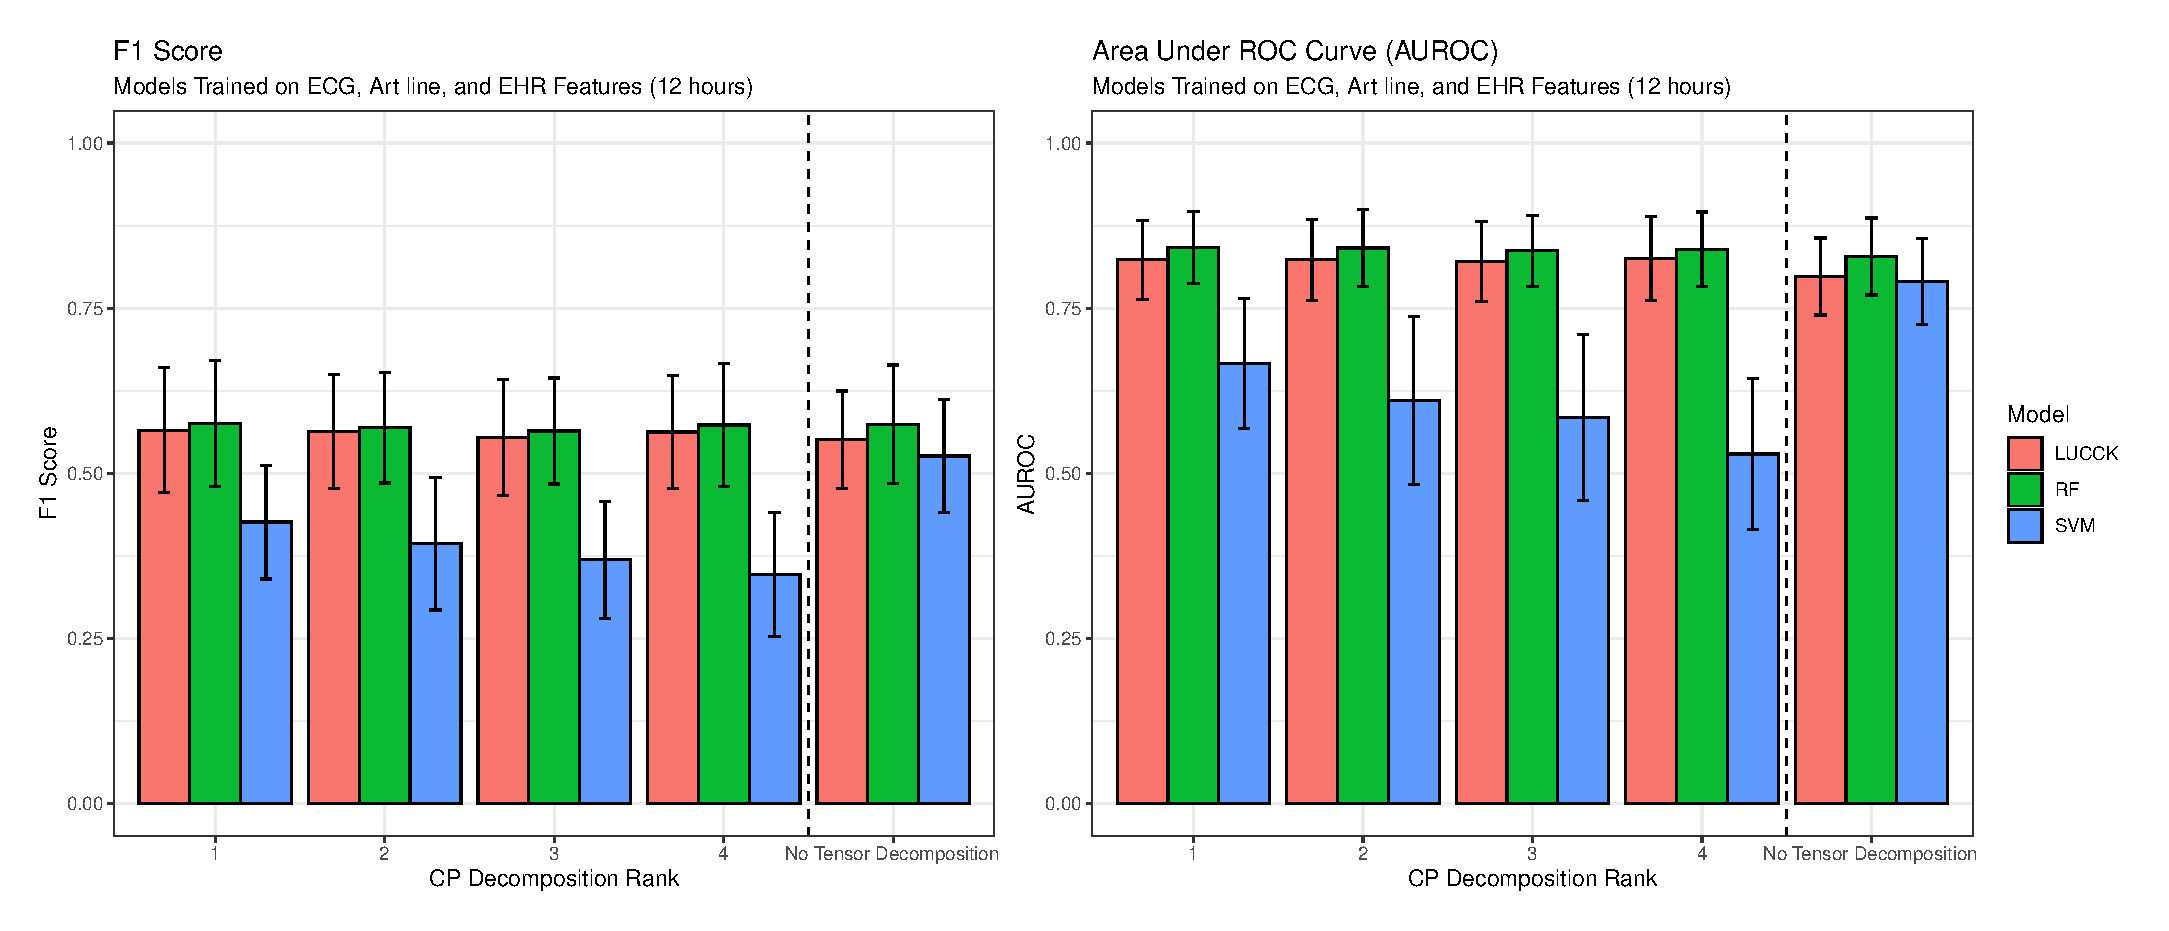
\includegraphics[width=\textwidth]{body/figures/all_12.eps}
        \caption{12-hour data}
    \end{subfigure}
    \caption{Models Trained with Arterial Line, ECG, and EHR Data}
    \label{fig:sigEHR}
\end{figure}  % ART + ECG + EHR 

\clearpage